\chapter{Visual-inertial SLAM with fiducial markers}
\label{chp:absolute_vi}
\minitoc
\bigskip

Results presented in this section are adapted from our published work \cite{fourmy2019absolute}. The opinions and perspectives reflected are the ones we had
at the time.

\section{Introduction}

In this work, we are interested in quantifying how accurately a humanoid robot can be localized in a structured 3D environment.
The seminal works on localization of legged robots were using leg odometry \cite{roston1991dead}, quickly followed by contributions fusing the kinematics 
with inertial measurements~\cite{lin2006sensor}. Naturally, odometry measurements can only lead to a drift of the localization.
Based on leg odometry, the community has extended the localization performances by improving the behavior of the inertial-kinematic 
filter~\cite{bloesch2013state,rotella2014state,flayols2017experimental}, the underlying contact 
model~\cite{bledt2018cheetah,rotella2018unsupervised}, and by augmenting the odometer with exteroceptive measurements coming from cameras 
or LIDAR \cite{stasse2006real, fallon2014drift, camurri2017multisensory}.

The difficulty in fusing inertial, kinematics, and exteroceptive measurements stems from the disparity in the properties of each data source.
Inertial and kinematic measurements come at high frequency (typically 100 Hz to 1 kHz) and are cheap to process, while images and laser scans 
are obtained at some few images per second and are expensive to process. 
On the other hand, inertial measurements are quickly deprecated while images and scans provide absolute information.
This implies a rigorous synchronization between the sensors with the risk of decreasing the performances of the inertial 
estimation when images and laser scans are not carefully merged. 

These difficulties explain that the first works to merge proprioceptive and exteroceptive sensors for legged localization 
have been with staggered approach, first fusing inertial and kinematic measurements at high frequency, and then correcting 
the localization drift with absolute localization computed the from the camera and/or the LIDAR with low bandwidth and higher 
delay~\cite{nobili2017heterogeneous,fallon2014drift}.

Very recently, several concurrent approaches have been proposed to merge all relevant data in a unique estimator.
Following the recent results in UAVs localization~\cite{forster2017-TRO,leutenegger2015keyframe}, optimal estimation 
structured by a factor graph seems to be an suitable framework to formulate the fusion.
In~\cite{hartley2018legged}, a graph-SLAM is proposed to fuse inertial, kinematics, and visual data.
Inertial measurements are considered using Forster's pre-integration factors~\cite{forster2017-TRO}, which is recalled in \secRef{sec:imu_preint_composite}.
Kinematics data are included using a 6D factor which is also pre-integrated, taking into account the hybrid nature 
of the contact dynamics using an event-based approach.
Visual factors are also expressed as 6D factors obtained by visual odometry. Results are reported on sequences of a few meters with motion-capture ground-truth.
In~\cite{wisth2019robust}, the graph-SLAM also considers inertial measurements through Forster's pre-integration, while kinematic
 measurements are pre-treated by the robot low-level system~\cite{bloesch2017two} and integrated directly as 6D factors without further consideration.
% As this work is applied to a quadruped robot, obtaining this 6D information indeed requires complex filtering in itself. 
Finally, the visual information is included as 2D pixel reprojection factors in the image space, obtained from feature tracking (KLT \cite{baker2004lucas}).
Impressive experimental results are demonstrated with long outdoor sequences, using a ground-truth obtained from off-line LIDAR reconstruction.

The pros and cons of these two approaches come from the choice of the factors, but the similarities are possibly more important than the differences.
Both use a plain Forster pre-integration~\cite{forster2017-TRO}. 
Using either visual odometry or feature tracking, both systems cannot natively benefit from the information brought by loop closure and would fail 
to exploit known map information.
In both cases, the kinematic factor is straightforward to write as a 6D probabilistic constraint.
Finally, both works can account for the very different sensor frequencies, while providing a good estimate at the higher frequency if needed.


\begin{figure}[h]
    \centering
    \begin{subfigure}{0.384\textwidth}
        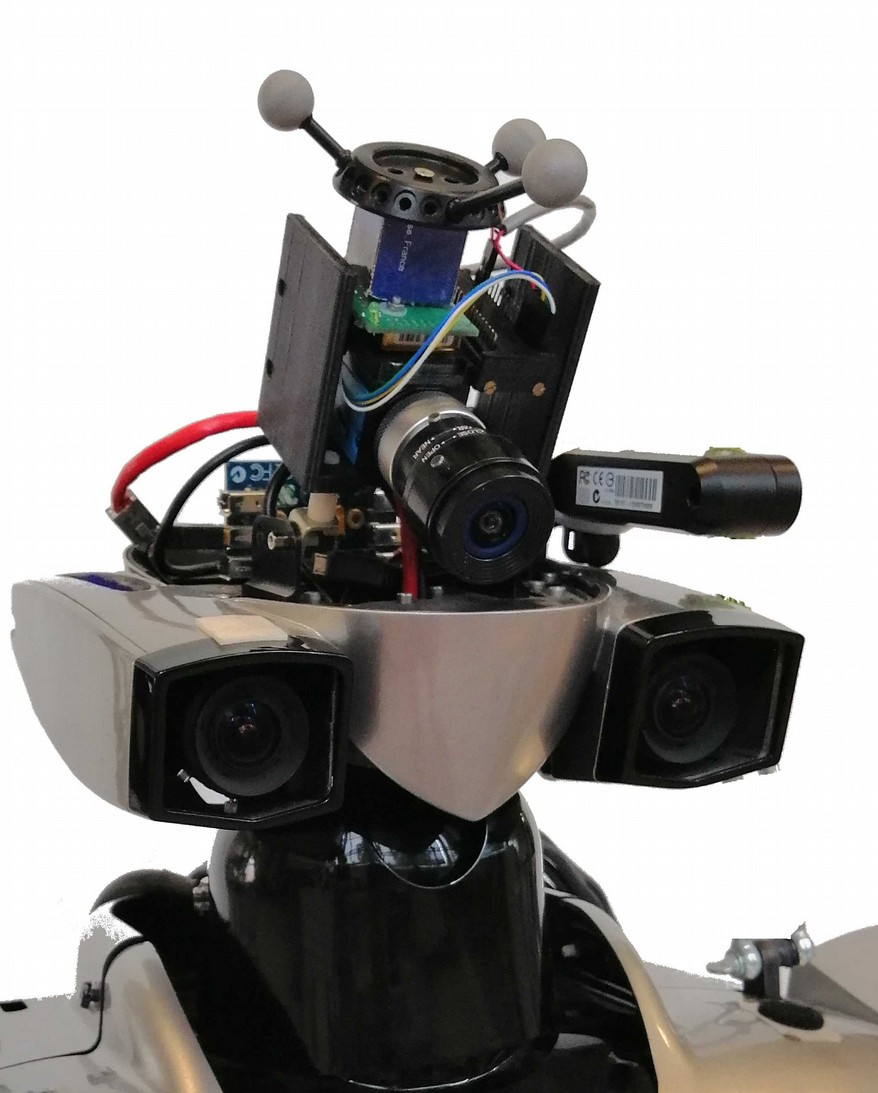
\includegraphics[width=\textwidth]{figures/absolute/HPR2_head_crop.png}
        \caption{HRP2 robot with which were conducted the experiments. The head was replaced by our visual-inertial sensor.}
        \label{fig:HPR2_head_crop}
    \end{subfigure}
    \hfill
    \begin{subfigure}{0.546\textwidth}
        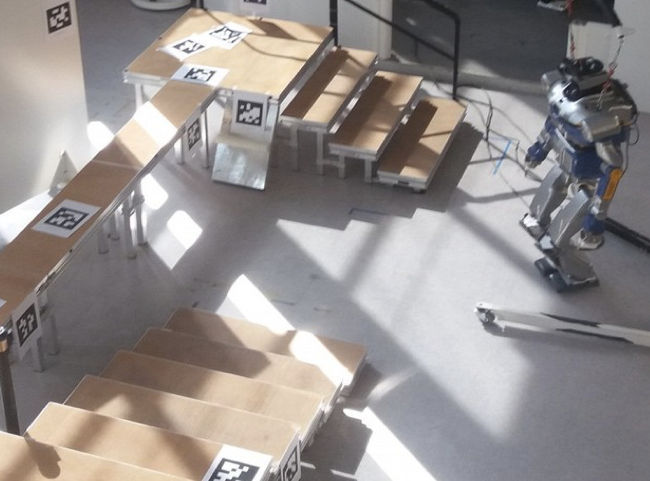
\includegraphics[width=\textwidth]{figures/absolute/bauzil.png}
        \caption{Experimental room with parkour, \HRP{2} and fiducial markers.}
    \end{subfigure}
    \label{fig:bauzil}
    \caption{Experimental setup. (\subref{fig:HPR2_head_crop}): installation of the visual-inertial sensor. (\subref{fig:bauzil}): experimental space.}
    \label{fig:HRP2}
\end{figure}

In this work, we are looking for a solution to localize a humanoid robot indoors, with sufficient accuracy to navigate on some stairs, grasp a handrail, or 
walk on a 30-cm wide beam. 
As the robot is going to come back again and again in the same environment, we would like to benefit from loop-closure information and localization with 
respect to some known landmarks. 
While our final goal is to merge in the optimal estimator the measurements coming from all the sensors of the robot, we focus here on contributions 
validating the use of visual-inertial localization and mapping on a humanoid robot navigating indoors in a 3D environment.
For the visual factor, we rely on \apriltags \cite{wang2016iros}, while proposing a practical contribution to avoid ambiguity 
issues in the pose estimation of the tags, as described in \secRef{sec:fiducial_markers}. 
For the inertial factor, we build upon Forster pre-integration~\cite{forster2017-TRO} and propose an original,% and more rigorous theoretical formulation, 
by exhibiting a compact Lie group (described in \secRef{sec:imu_preint_compact}) that is suitable for optimal estimation. 
This formulation, although leading to very similar formulas % results -> we don't have practical results to compare 
for the inertial factors, enables a generalization to the other high-frequency factors 
that would typically arise in the humanoid contact (leg odometry based on coders, force sensors, etc).
Both inertial and visual factors are processed in a factor graph resulting in a nonlinear least-square optimization problem, solved with Ceres~\cite{ceres-solver}.

In the following section, we first formalize the inertial SLAM estimation problem that we wish to solve. Then we present experimental results on datasets obtained
with a visual-inertial sensor (VIS) carried by a human operator and the \HRP{2} humanoid robot. 



\section{Problem statement}

\begin{figure}
    \centering
    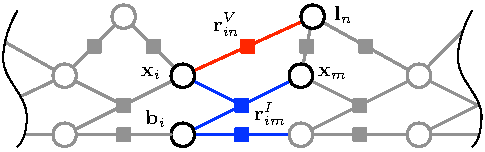
\includegraphics[scale=1.3]{figures/absolute/graph}
    \caption{A typical fraction of the factor graph, involving state blocks corresponding to keyframes $\bfx_i=(\bfp_i,\bfv_i,\bfR_i)$, biases $\bfb_i$ and landmark poses $\bfl_n$. 
    IMU factors (blue) relate consecutive keyframes and the IMU biases.
    The lower branch controls bias drift along time.
    Visual factors (red) relate landmarks with poses $(\bfp_i,\bfR_i)$.}
    \label{fig:graph}
\end{figure}

In graph-based optimization, the problem is well represented as a bipartite graph, where one type of node refers to the variables, 
and the other type called \emph{factors} represents probabilistic constraints between variables, produced by the measurements.
%
% The state $\bfx$ is modeled as a multi-variate Gaussian distribution.
In the case of landmark-based visual-inertial SLAM (see \figRef{fig:graph}), $\bfx$ includes robot poses and velocities 
$\bfx=(\bfp,\bfv,\bfR)$ and IMU biases $\bfb$, both at selected \keyframes\ along the trajectory, and landmark poses $\bfl \in \SE(3)$.
Biases are considered constant between \keyframes\.
%
In line with the recent works on the subject, we write the MAP optimization as the least-squares minimization (\figRef{fig:graph}),
%
\begin{align}\label{equ:least_squares}
    \cX^* = \argmin_\cX 
    \sum_i \norm{\bfr^I_i(\cX)}_{\Cov^I_i}^2
    +
    \sum_j \norm{\bfr^V_j(\cX)}_{\Cov^V_j}^2
    % +
    % \sum_c \norm{\bfr_c(\bfx)}_{\Sigma_c}^2
~,
\end{align}
%
with $\{\bfr^I,\Cov^I\}$ and $\{\bfr^V,\Cov^V\}$ indicating the residuals and covariances of respectively the inertial (IMU) and visual factors.
These residuals are computed differently depending on the nature of the measurements and the state blocks they relate to. 
The \apriltag\ factor is described in this thesis \chpRef{chp:object_level} and the IMU factor in \chpRef{chp:preintegration}.


\section{Results}

\subsection{Experimental setup}
We have gathered several datasets in the experimental arena of the humanoid robots at LAAS-CNRS, a 3D environment about $10m \times 5m$ made of flat floor, 
stairs, and a 30cm wide beam.
The robot environment was augmented with about 20 fiducial ``\apriltag'' markers (of about 20 cm width).
The tags have been randomly dispatched in the environment.
They are fixed during a run but may vary significantly between two sets of data, and their locations are not calibrated ---that is, we do not have ground-truth localization of the tags.

Each dataset is composed of 3 sequences:
\begin{itemize}
    \item a sequence of RGB images captured at 33 Hz
    \item a sequence of IMU measures captured at 200 Hz
    \item a sequence of motion-capture (MoCap) at 200Hz measurements used as ground-truth.
\end{itemize}


\begin{figure}[t]
    \centering
    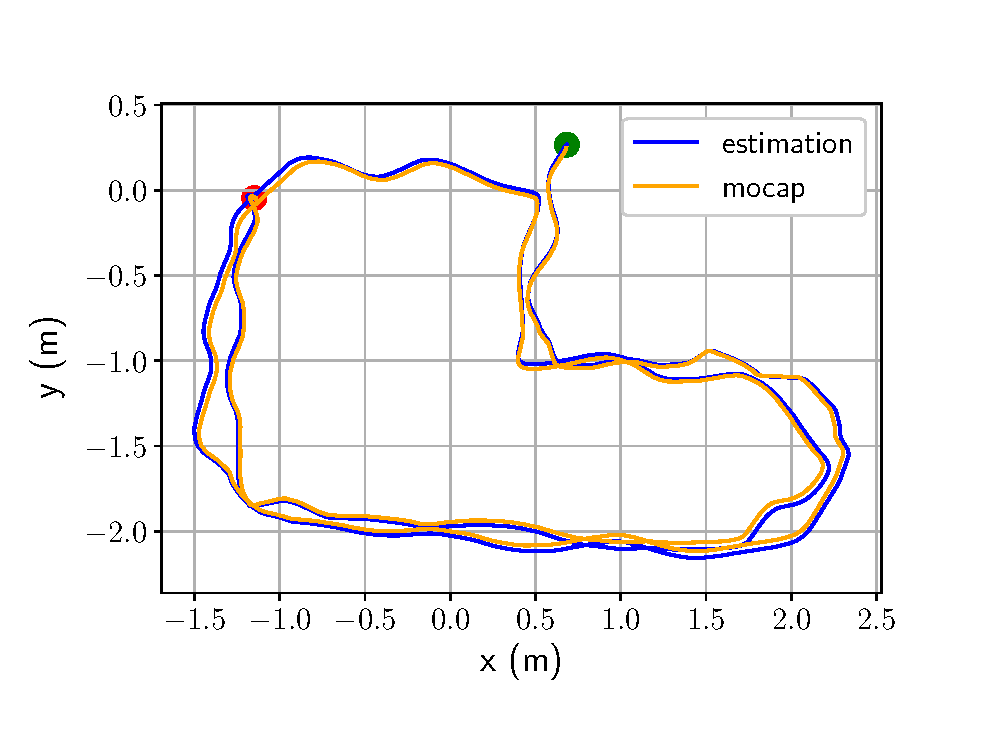
\includegraphics[scale=0.8]{figures/absolute/xy_loop_twice.eps}
    \caption{Two loops of the experimental field with camera in hand}
    \label{fig:xy_loop_twice}
\end{figure}

%
\begin{table}[t]
    \centering
    \caption{Datasets description and results}
    \begin{tabular}{c|c|c|c|c}
        Description & Duration & Length & MTE$^1$ & STE$^2$ \\
        \hline
        \hline
        Handheld loop & 59.0\,\textrm{s} & 20.6\,\textrm{m} & 29.0 & 11.3  \\
        \hline
        HRP2 turns then walks & 59.9\,\textrm{s} & 12.87\,\textrm{m} & 30.9 & 15.7 \\
        \hline
        HRP2 climbs stairs & 47.1\,\textrm{s} & 6.25\,\textrm{m} & 13.9 & 6.3 \\
        \hline
        HRP2 descends stairs & \, 19.39\textrm{s} & \, 2.62\textrm{m} & 30.4 & 11.8 \\
        \hline
        \multicolumn{5}{l}{$^1$ Mean translation error [mm]} \\
        \multicolumn{5}{l}{$^2$ Std. dev. of translation error [mm]} 
    \end{tabular}
    \label{tab:datasets}
\end{table}


The visual-inertial sensor (VIS) is comprised of a Memsic IMU running at 200 Hz and an Imagine Source camera.
IMU and camera are hardware synchronized: the image acquisition is triggered by a micro-controller (STM32) synchronized with the IMU.
We have validated that there is less than a 2 ms synchronization error by the hardware (shutter time) and that this delay is stable.
The camera and the IMU are collocated, with less than 10 cm of distance between IMU and camera focal. 
The camera-to-IMU extrinsics parameter was calibrated using the Kalibr library \cite{furgale2013unified}.
% Although our implementation of the least-squares estimator can handle sensor calibration, we have not tried to calibrate the camera-to-IMU extrinsic parameters online.
In each sequence, we have taken care that the camera is navigating in a comfortably-dense field of tags, even if it may not have always a tag in its field of view.
The motion-capture data have been obtained from a calibrated 3D marker attached to the camera and are synchronized in post-process by maximizing the velocity norm 
cross-correlation between MoCap and estimated state sequences.
% The datasets are available at \url{https://gepgitlab.laas.fr/loco-3d/wolf-data/}.
%In order to gather datasets to test our estimator, we designed a Visual Inertial System (VIS) comprised of a Memsic IMU running at 200Hz synchronized through a 
% micro-controller (STM32) with an Imagine Source camera which captures are hardware triggered. Noises parameters of the IMU were estimated using the 
% Allanvariance method described in \cite{el2007analysis}.
%We recorded several datasets in which the camera was either handheld or mounted on the head of a HRP2 humanoid robot. Rosbags for the datasets are available at 
% [url]. Ground truth is also provided thanks to a [brand name] motion capture system (mocap) recording the system pose at 200Hz.
%
\begin{figure}[t]
     \centering
     \begin{subfigure}{0.5\textwidth}
         \centering
         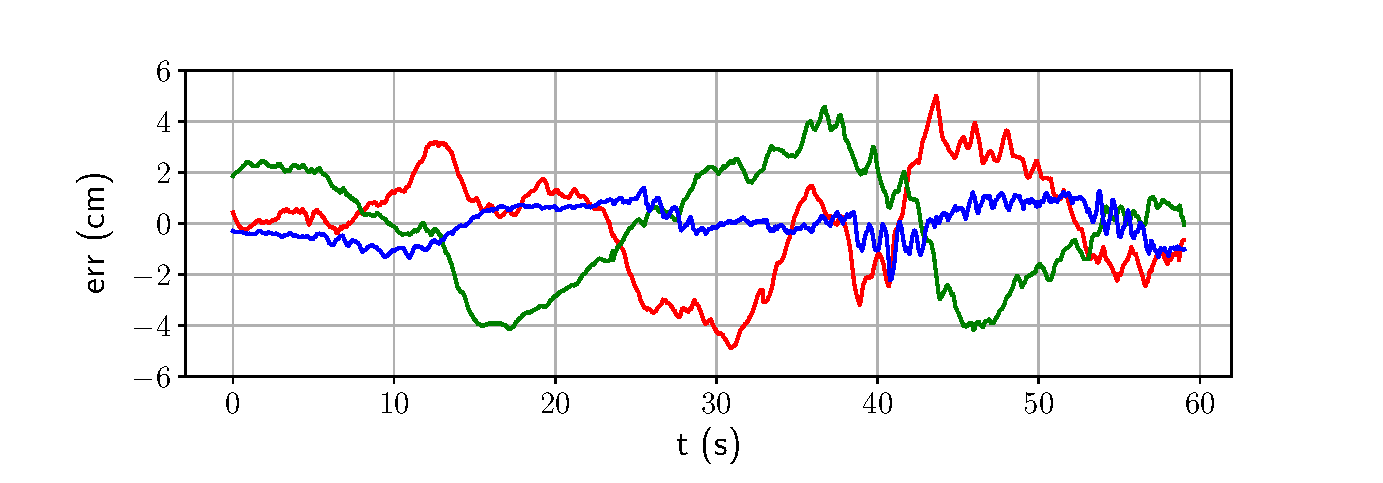
\includegraphics[width=\textwidth]{figures/absolute/terr_loop_twice.eps}
     \end{subfigure}%
     \hfill
     \begin{subfigure}{0.5\textwidth}
         \centering
         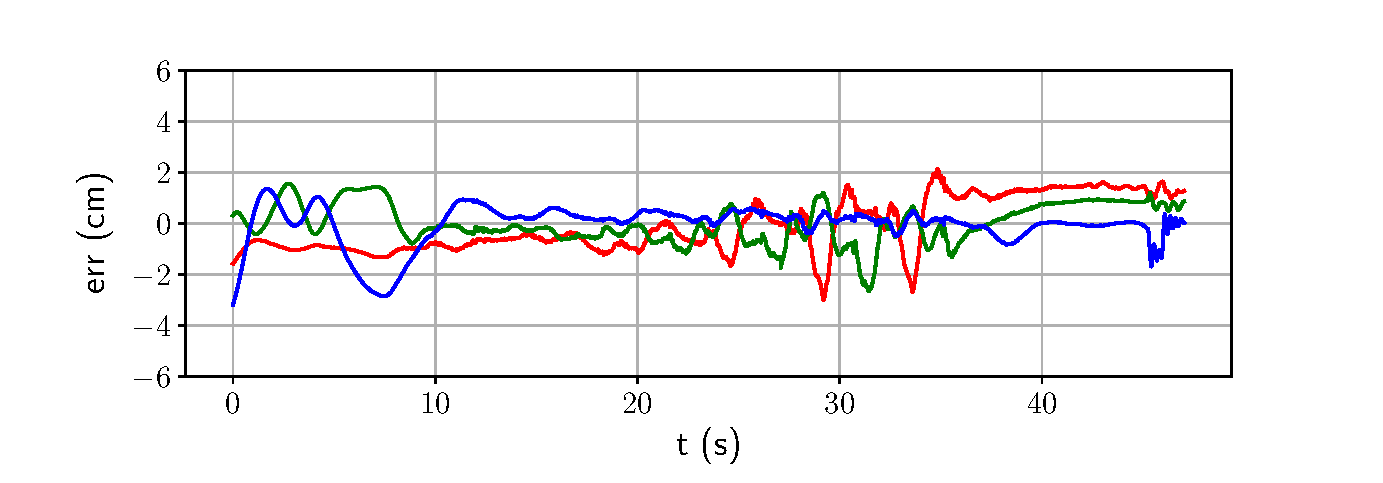
\includegraphics[width=\textwidth]{figures/absolute/terr_stairs1.eps}
     \end{subfigure}%
     \\
    \begin{subfigure}{0.5\textwidth}
         \centering
         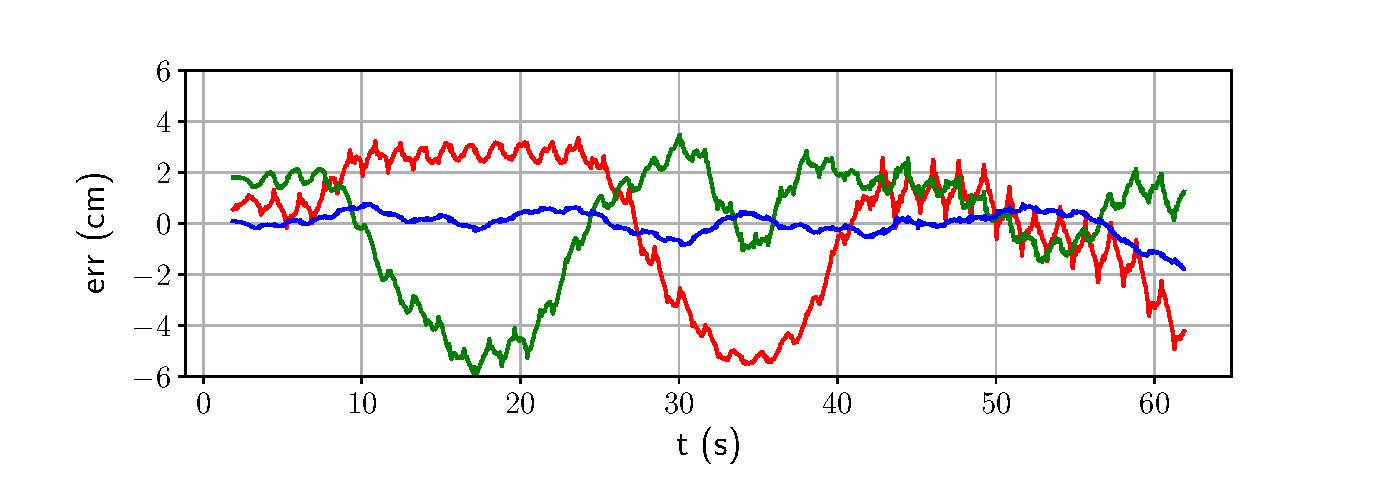
\includegraphics[width=\textwidth]{figures/absolute/terr_robot1_walking.eps}
     \end{subfigure}%
     \hfill
     \begin{subfigure}{0.5\textwidth}
         \centering
         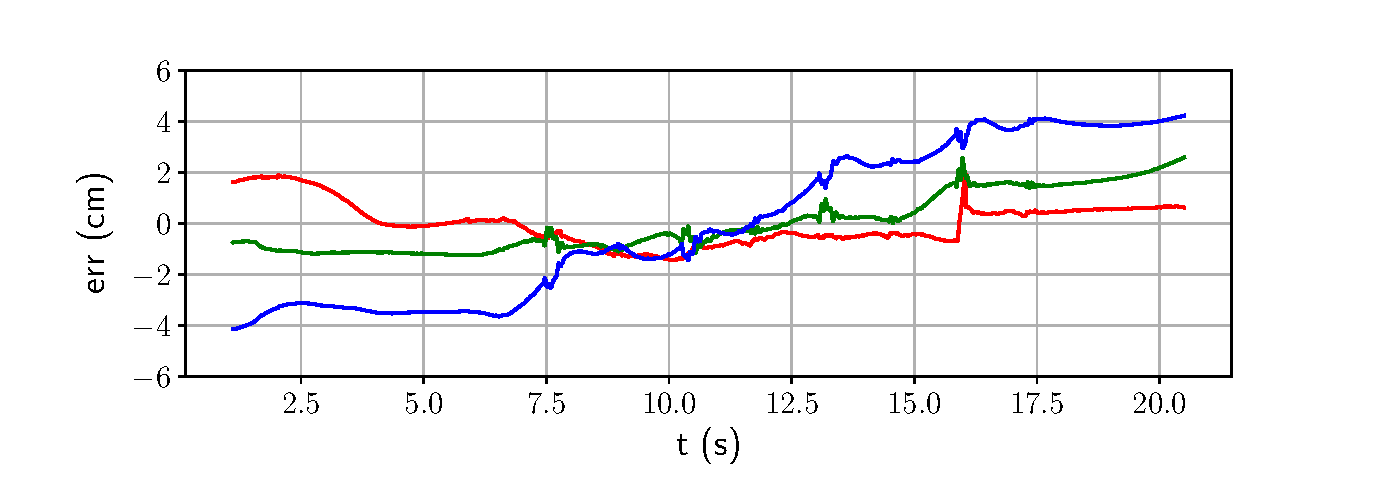
\includegraphics[width=\textwidth]{figures/absolute/terr_descending2.eps}
     \end{subfigure}%
    \caption{Translation estimation error (cm) as a function of time (s). In the clock-wise sens, starting from the 
             top-left corner, the datasets are handheld camera, stairs climbing, stairs descending and walking on flat ground. 
             RGB colors correspond to xyz axes.}
    \label{fig:results}
\end{figure}


\subsection{Localization precision}

We consider four datasets that are summarized in table \tabRef{tab:datasets}. They cover different tasks on which a consistent 
estimation of the robot movement is necessary. The first one is a relatively long sequence consisting of two loops with the VIS handheld. 
This is used to test the long-term localization of the robot, which is interesting for navigation. Secondly, we made the LAAS Gepetto team 
\HRP{2} walk and turn around on a short distance to evaluate the resilience of the filter to the vibrations of the robot. Finally, two more 
challenging datasets are recorded while the robot is climbing and descending stairs. Especially on the latter, the locomotion causes impacts 
that on one hand bring the IMU close to its dynamic range saturation, and on the other hand, provoke images with motion blur. Note that during these experiments, 
the estimator was not used for feedback control. To compare our results with the ground-truth, we used methods described in \cite{zhang2018tutorial} to align 
trajectories given that 4 DoFs are unobservable in VI estimation.
For each case, \keyframes\ are created at a frequency of 6.6 Hz (every 5 images) if tags are detected in the corresponding image.

\begin{figure}[h]
    \centering
    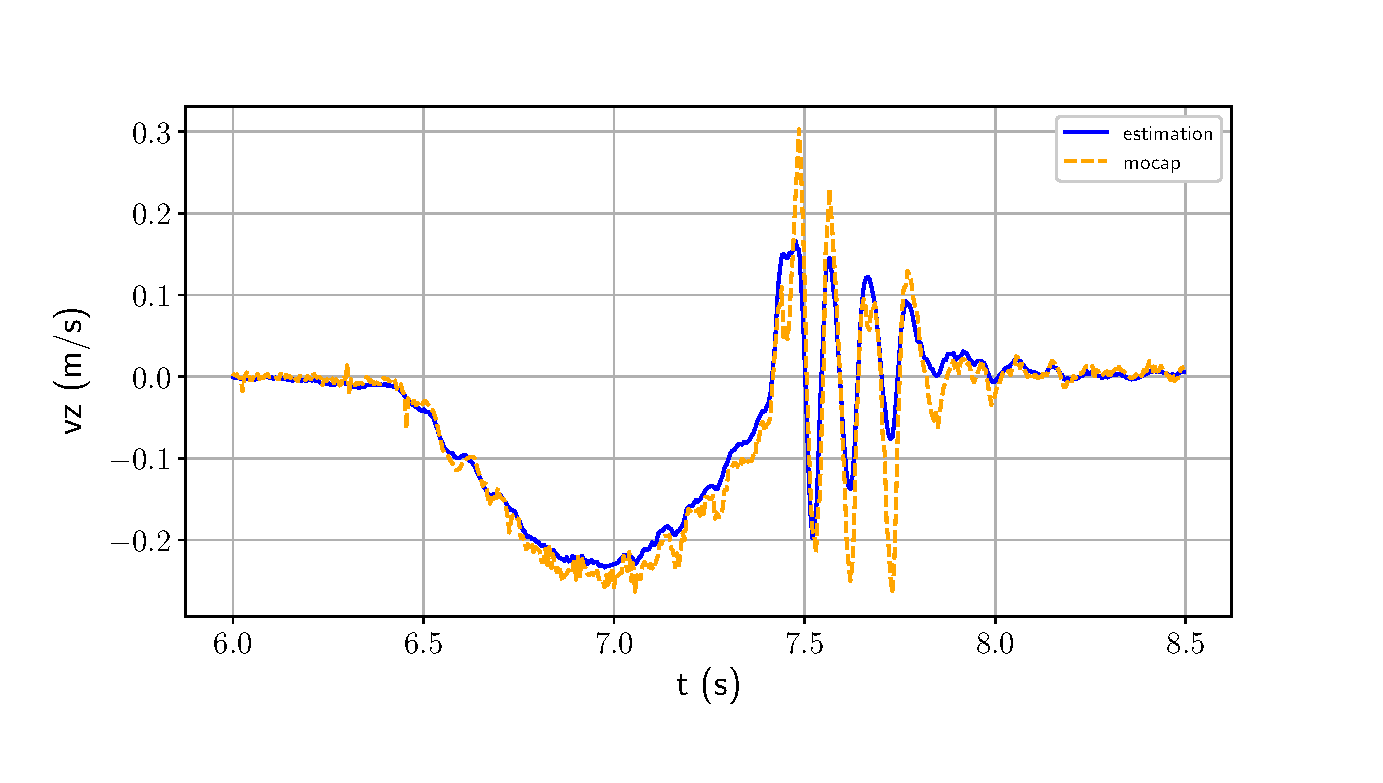
\includegraphics[width=0.8\textwidth]{figures/absolute/vz_descending_onestep.eps}
    \caption{Descending stairs (one step): the robot first lowers its center of mass and then touches the next step with results in vibrations from the impact.}
    \label{fig:vz_descending_onestep}
\end{figure}

\figRef{fig:results} presents a quantitative evaluation of the translational errors. In all cases, our estimator achieves errors consistently below a few centimeters. 
The biggest errors are obtained for the walking datasets where the two humps correspond to phases where the robot is turning on itself and sees landmarks that will not be 
seen again later in the trajectory.

A high rate estimation of a humanoid robot velocity and in particular of its center of mass is critical for balance controllers. It can be recovered from motion capture through numerical differentiation of the positions, but this results in a quite noisy time series. It is especially visible when hard impacts make the robot shake at approximately 10 Hz. 
The estimated velocity follows a familiar oscillatory damped system behavior while the mocap estimation is more erratic. 
%In this sense, our estimator seems to be more fit for feedback control than the use of the MoCap.


\subsection{Related works}
Two \apriltag\ based visual-inertial SLAM systems have been implemented in the previous years. 
In \cite{neunert2016open}, the authors rely on an EKF in which state propagation is naturally 
handled by the IMU and each marker detection is used in an update step where the reprojection error of its 4 corners provides an 8D innovation vector. 
A closer solution to ours was very recently proposed in \cite{he2019lightweight} and is also based on graph SLAM optimization benefiting from 
Forster's IMU pre-integration from GTSAM. As explained previously, the \apriltag\  factor formulation is different from ours and the algorithm is tested 
on large datasets consisting only of smooth motions.
